\documentclass[]{elsarticle} %review=doublespace preprint=single 5p=2 column
%%% Begin My package additions %%%%%%%%%%%%%%%%%%%
\usepackage[hyphens]{url}
\usepackage{lineno} % add
\providecommand{\tightlist}{%
  \setlength{\itemsep}{0pt}\setlength{\parskip}{0pt}}

\bibliographystyle{elsarticle-harv}
\biboptions{sort&compress} % For natbib
\usepackage{graphicx}
\usepackage{booktabs} % book-quality tables
%% Redefines the elsarticle footer
%\makeatletter
%\def\ps@pprintTitle{%
% \let\@oddhead\@empty
% \let\@evenhead\@empty
% \def\@oddfoot{\it \hfill\today}%
% \let\@evenfoot\@oddfoot}
%\makeatother
\renewcommand*{\today}{December 5, 2016}

% A modified page layout
\textwidth 6.75in
\oddsidemargin -0.15in
\evensidemargin -0.15in
\textheight 9in
\topmargin -0.5in
%%%%%%%%%%%%%%%% end my additions to header

\usepackage[T1]{fontenc}
\usepackage{lmodern}
\usepackage{amssymb,amsmath}
\usepackage{ifxetex,ifluatex}
\usepackage{fixltx2e} % provides \textsubscript
% use upquote if available, for straight quotes in verbatim environments
\IfFileExists{upquote.sty}{\usepackage{upquote}}{}
\ifnum 0\ifxetex 1\fi\ifluatex 1\fi=0 % if pdftex
  \usepackage[utf8]{inputenc}
\else % if luatex or xelatex
  \usepackage{fontspec}
  \ifxetex
    \usepackage{xltxtra,xunicode}
  \fi
  \defaultfontfeatures{Mapping=tex-text,Scale=MatchLowercase}
  \newcommand{\euro}{€}
\fi
% use microtype if available
\IfFileExists{microtype.sty}{\usepackage{microtype}}{}
\usepackage{longtable}
\usepackage{graphicx}
% We will generate all images so they have a width \maxwidth. This means
% that they will get their normal width if they fit onto the page, but
% are scaled down if they would overflow the margins.
\makeatletter
\def\maxwidth{\ifdim\Gin@nat@width>\linewidth\linewidth
\else\Gin@nat@width\fi}
\makeatother
\let\Oldincludegraphics\includegraphics
\renewcommand{\includegraphics}[1]{\Oldincludegraphics[width=\maxwidth]{#1}}
\ifxetex
  \usepackage[setpagesize=false, % page size defined by xetex
              unicode=false, % unicode breaks when used with xetex
              xetex]{hyperref}
\else
  \usepackage[unicode=true]{hyperref}
\fi
\hypersetup{breaklinks=true,
            bookmarks=true,
            pdfauthor={},
            pdftitle={In-Depth Analysis of Interreader Agreement and Accuracy in Categorical Assessment of Brown Adipose Tissue in (18)FDG-PET/CT},
            colorlinks=true,
            urlcolor=blue,
            linkcolor=magenta,
            pdfborder={0 0 0}}
\urlstyle{same}  % don't use monospace font for urls
\setlength{\parindent}{0pt}
\setlength{\parskip}{6pt plus 2pt minus 1pt}
\setlength{\emergencystretch}{3em}  % prevent overfull lines
\setcounter{secnumdepth}{0}
% Pandoc toggle for numbering sections (defaults to be off)
\setcounter{secnumdepth}{0}
% Pandoc header


\usepackage[nomarkers]{endfloat}

\begin{document}
\begin{frontmatter}

  \title{In-Depth Analysis of Interreader Agreement and Accuracy in Categorical
Assessment of Brown Adipose Tissue in (18)FDG-PET/CT}
    \author[University Hospital of Zurich]{Anton S. Becker, M.D.\corref{c1}}
   \ead{anton.becker@usz.ch} 
   \cortext[c1]{Corresponding Author}
    \author[University Hospital of Zurich]{Caroline Zellweger, M.D.}
  
  
    \author[University Hospital of Zurich]{Khoschy Schawkat, M.D.}
  
  
    \author[University Hospital of Zurich]{Sanja Bogdanovic, M.D.}
  
  
    \author[University Hospital of Zurich]{Valerie Doan Phi van, M.D.}
  
  
    \author[University Hospital of Zurich]{Hannes W. Nagel, M.D.}
  
  
    \author[ETH Zurich]{Christian Wolfrum, Ph.D.}
  
  
    \author[University Hospital of Zurich]{Irene A. Burger, M.D.}
  
  
      \address[University Hospital of Zurich]{University Hospital of Zurich, Raemistrasse 100, Zurich, Switzerland}
    \address[ETH Zurich]{ETH Zurich, Universitaetsstrasse 2, 8092 Zurich}
  
  \begin{abstract}
  \emph{Purpose} To evaluate the interreader agreement of a three-tier
  craniocaudal grading system for brown fat activation and investigate the
  accuracy of the distinction between the three grades.
  
  \emph{Materials and Methods} After IRB approval, 340 cases were
  retrospectively selected from patients undergoing (18)FDG-PET/CT between
  2007-2015 at our institution, with 85 cases in each grade and 85
  controls with no active brown fat. Three readers evaluated all cases
  independently. Agreement between the readers was assessed with Cohen's
  Kappa (k), the concordance correlation coefficient (CCC) and the
  intraclass correlation coefficient (ICC). Accuracy was assessed with
  Bland-Altman and receiver operating characteristics (ROC) analysis. A
  Bonferroni-corrected two-tailed p\textless{}0.016 was considered
  statistically significant.
  
  \emph{Results} Agreement was excellent by all three metrics with k =
  0.83-0.89, CCC = 0.83-0.89 and ICC = 0.91-0.94. Bland-Altman analysis
  revealed only slight average over- or underestimation (-0.01-0.14) with
  the majority of disagreements within one grade. ROC analysis yielded
  slightly less accurate classification between higher vs.~lower grades
  (Area under the ROC curves 0.78-0.84 vs.~0.88-0.92) but no significant
  differences between readers.
  
  \emph{Conclusion} Grading the activation of brown fat by assessment of
  the most caudally activated depots results in excellent interreader
  agreement, comparable to previously reported agreement using SUV
  measurements.
  \end{abstract}
  
 \end{frontmatter}

\emph{This is a preprint version (before peer-review) of the original
paper: 10.1016/j.ejrad.2017.03.012}

\subsection{Introduction}\label{introduction}

Obesity has become a serious health problem worldwide. Despite all
efforts, obesity is still on the rise globally and the prevalence will
surpass 18\% in men and 21\% in women after 2025 {[}1{]}. Chronic
obesity entails several co-morbidities such as type II diabetes,
atherosclerotic changes, early osteoarthritis and some types of cancer
{[}2{]}. Although various approaches have been undertaken to fight
obesity, for example, but not limited to, lifestyle modification or
pharmacologic therapy these attempts have, at best, yielded modest
results {[}3,4{]}. For this reason, the initial discovery of
metabolically active brown adipose tissue (`brown fat') in adult humans
in 2002 {[}5{]} and the subsequent description in a larger human cohort
seven years later {[}6,7{]} has sparked an active field of research on
how to exploit its ``calorie burning properties'' to facilitate weight
loss. The main function of brown fat, as opposed to white fat, which
stores excess energy in the form of triacylglycerols, is the dissipation
of energy into heat. For this purpose triacylglycerols, amino acids or
glucose can be utilized. Thanks to the latter substrate, brown fat can
be detected in-vivo by (18)FDG-PET/CT due to its ability to precisely
match functional metabolic with spacial anatomic information. To date,
(18)FDG-PET hybrid imaging with CT or MRI is the only medical imaging
modality able to do so. Beyond detection, (18)FDG-PET also allows
quantification of glycolytic activity in standarized uptake values
(SUV). This is of paramount importance in order to be able to evaluate
new therapeutic approaches. Bahler and colleagues have recently
demonstrated excellent interreader agreement of brown fat SUV
measurements {[}8{]}. However, the measurement process of brown fat
tends to be cumbersome and time-consuming because other glycolytic
tissues (myocardium, liver, muscle) need to be manually cropped from the
volume of interest. Albeit there are interesting approaches to automate
this process such as the one presented by Gifford et al. {[}9{]}, they
are usually fairly complicated per-se and not readily available.
Moreover, specialized software is needed which is usually associated
with high costs and a steep learning curve. Recently, it was shown that
more caudal activation of brown fat correlates with all glycolytic
measures: SUV\textsubscript{max}, metabolic active volume as well as
total brown fat activity {[}10{]}, which led to the proposal of a
three-tier grading system based on the most caudally activated brown fat
depot. Such a system allows for faster classification on a standard
radiology workstation. Especially for the analysis of larger cohorts
this could substantially simplify read outs. However, it is not clear
what impact such a grading system will have on the interreader
agreement. The binning of continuous SUV measurements, which are very
reliable {[}8{]}, into discrete categories could theoretically lead to
more pronounced disagreement. Thus, the purpose of this study was to
evaluate the interreader agreement of the three-tier craniocaudal
grading system and investigate the accuracy of the readers for the
distinction between the three grades.

\subsection{Materials and Methods}\label{materials-and-methods}

This retrospective study was approved by the IRB, who waived the need
for informed consent.

\subsubsection{FDG-PET/CT protocol}\label{fdg-petct-protocol}

All scans had been acquired as routine clinical examinations. In
summary, patients were instructed to fast for at least 6h prior to the
examination. Fasting blood glucose was verified to be below
\textless{}7mmol/L. After injection of 4 mBq FDG per kilogram
bodyweight, patients were laid with closed eyes in supine position in a
quiet, even-tempered room. After 60 minutes (±5 min.) a low-dose CT scan
was acquired (120--140 kV, mAs dynamically regulated by SmartmA (R)),
followed by the PET scan from mid-thigh to the vertex of the skull.

\subsubsection{Grading System}\label{grading-system}

The activation strength of the brown fat was divided into four
categories according to the grades proposed by {[}10{]}: 0 = no active
brown fat, 1 = nuchal and/or supraclavicular, 2 = thoracic, 3 =
infradiaphragmal fat depots activated, as illustrated in \emph{Figure
1}.

\subsubsection{Patient Population}\label{patient-population}

In a retrospective analysis of roughly 8300 patients undergoing
FDG-PET/CT in the years 2007-2015, metabolically active brown fat was
detected in 758 patients. Metabolically active brown fat was defined as
fat density tissue on CT (-250 to -50 Hounsfield Units) with a
corresponding SUV\textsubscript{max} of \textgreater{}2.5 g/ml. All
cases were classified according to the abovementioned three-tier
anatomical grading system. From each category 85 cases were randomly
selected, resulting in 340 cases.

\subsubsection{Readout}\label{readout}

One reader who had performed the initial screening and readout of all
PET/CT examinations (ASB) served as a reference standard. Three readers
who were blinded to the patient selection independently performed the
readout on a standard radiological worksataion (IMPAX, AGFA HealthCare
Inc., Bonn, Germany): KS (4th year radiology resident, no prior
experience in PET/CT), SB (1st year radiology resident, completed a
four-month rotation in PET/CT) and CZ (board certified radiologist, 2
years experience in PET/CT). Prior to the readout four cases not
included in the study population were evaluated as training cases. An
instruction sheet with a schematic similar to \emph{Figure 1} was
available during the readout.

\subsubsection{Statistical Analysis}\label{statistical-analysis}

Statistical Analysis was performed in R version 3.3.2 (R Core Team
(2016). R: A language and environment for statistical computing. R
Foundation for Statistical Computing, Vienna, Austria;
http://www.R-project.org/). Graphs were produced with ggplot2 {[}11{]}.
The full data and analysis are available in an online repository at
https://github.com/ASBecker/BAT-IRR.

\paragraph{Interreader agreement}\label{interreader-agreement}

Interreader agreement for all reader-pairs was investigated with Cohen's
weighted kappa (k), which accounts for agreements by chance {[}12{]},
and with the concordance correlation coefficient (CCC) {[}13{]} and the
intraclass correlation coefficient (ICC) 2k {[}14{]}. Since all three
metrics are widely used in the radiological literature we opted to
calculate and report each to allow better comparability to other
studies, which commonly only use one. Scores were considered
significantly different if the 95\% confidence intervals (CIs) did not
overlap and valued as follows: slight (\textless{} 0.20), fair
(0.20--0.39), moderate (0.40--0.59), substantial (0.60--0.79), and
excellent (\textgreater{} 0.80) agreement.

\paragraph{Classification accuracy}\label{classification-accuracy}

The deviation from the reference classification was assessed with
Bland-Altman analysis. Classification accuracy between the subsequent
categories (0-1, 1-2 and 2-3) was assessed with a receiving operator
characteristics (ROC) analysis. The area under the ROC-curve
(A\textsubscript{z}) was compared with DeLong's nonparametric test
{[}15{]}. A p-value of \textless{} 0.016 (\textless{}0.05 with
Bonferroni correction for 3 combinations, two-tailed alpha) was
considered statistically significant.

\subsection{Results}\label{results}

All three readers completed the readout successfully for all 340 cases
(85 cases per category 1-3 and 85 controls).

\paragraph{Interreader agreement}\label{interreader-agreement-1}

Cohen's k suggested excellent agreement for all reader pairs and ranged
between 0.83 and 0.89 with all CIs overlapping, indicating no
substantial differences (\emph{Table 1}). The CCC yielded almost
identical results, with scores between 0.83 and 0.89 and no significant
differences (\emph{Table 2}). The ICC yielded the highest scores ranging
from 0.91 to 0.94 (\emph{Table 3}) with again no significant differences
between readers.

\paragraph{Classification accuracy}\label{classification-accuracy-1}

As described above, the original readout by BLINDED served as a
reference standard. Readers 1 and 2 seemed to slightly overestimate the
strength of brown fat activation with a mean difference of 0.07 and
0.14, however, the majority of different ratings did not exceed two
categories, as indicated by the dashed lines in \emph{Figure 2a} and
\emph{2b}. Reader 3 was closest to the reference standard with a slight
underestimation on -0.04 and also most differences one category above or
below the reference as shown in \emph{Figure 2c}. ROC analysis revealed
near-perfect brown fat detection for all three readers
(A\textsubscript{z} Reader 1 = 0.97, A\textsubscript{z} Reader 2 and 3 =
0.95). The classification accuracy was highest for the distinction
between categories 0 and 1 (A\textsubscript{z} 0.92, 0.88 and 0.89) and
decreased for categories 1 and 2 (A\textsubscript{z} 0.80, 0.84, 0.82).
In the categories 2 and 3 (the accuracy decreased further for readers 1
and 2 (A\textsubscript{z} 0.78) and was steady for reader 3
(A\textsubscript{z} 0.84), as depicted in \emph{Figure 3}. Differences
in accuracy among the readers were not significant in all cases
(p\textgreater{}0.07).

\subsection{Discussion}\label{discussion}

In the present study we have demonstrated that grading of brown fat
activity by assessing the most caudally activated depot results in
excellent interreader agreement. Neither overall performance nor
agreement was dependent on the experience of the reader, suggesting that
the grading system is suitable even for inexperienced radiologists.
However, the two less experienced readers tended to fare slightly worse
in the distinction between grade 2 and 3 brown fat activation. This is
not surprising since activity the suprarenal brown fat depot, which is
most often discriminative of grade 3, can be very subtle (false
negative, \emph{Figure 4a}) or mismatched with muscle activity from the
crus of the diaphragm (false positive, \emph{Figure 4b}). Moreover, the
depot tends to be fairly small in lean people, who are more inclined
towards higher levels of brown fat {[}6,7,10{]}.

In the radiological literature, three of the most widely used metrics
for assessing interreader agreement are Cohen's k {[}12{]}, CCC {[}13{]}
and ICC {[}14{]}. The latter is based on underlying ANOVA models, and
thus requires the assumption of equally distributed and randomly sampled
groups to be true. Although this was provided in our readout set, it may
not be given in other study populations and hence yield erroneous
results. Alternatively, the CCC is able to provide an estimate for
interreader agreement without underlying ANOVA assumptions. However,
with given ANOVA assumptions the CCC will yield very similar values to
the ICC, as was the case in the present study. Lastly, Cohen's k
assesses the agreement of ordinal (categorical) data while taking into
account agreement by chance. The weighted k furthermore makes a
distinction of how far the disagreements are apart in the case of
non-binary categories (m\textgreater{}2). However, it comes at the
expense of needing a rather large sample size in order to receive
reasonable confidence intervals (n=16m\^{}2 or n=256 in our case), as
determined by Chichetti and Fleiss {[}16{]} through Monte-Carlo
simulations. The k has another drawback of strongly depending on the
prevalence in the study population. This entails that e.g.~in a combined
detection-and-classification study with the usual observed
\textasciitilde{}10\% active brown fat prevalence, the k will be lower
because of the large likelihood of agreements by chance in the remaining
90\%. Hence, the CCC may be preferred over k in comparison between
different study populations.

Our results are in line with a previous report assessing interreader
agreement of SUV measurements of brown fat including
SUV\textsubscript{max}, SUV\textsubscript{mean} and volume {[}8{]}.
Though the CCC in the present study are slightly lower, they are not
unconditionally comparable as the underlying data is different
(continuous SUV versus categorical grade). Albeit SUV may appear to
offer a very precise measurement of metabolic activity, there are
several problems associated with it. First, as mentioned above, SUV
assessment requires specialized software and is cumbersome and time
consuming, whereas grading on a PACS workstation where the images are
readily available is a matter of seconds. Second, SUV vary depeding on
uptake time {[}17{]} and blood-glucose {[}18{]}, which are potential
confounders in retrospective (and multi-center) studies. Third, the
SUV\textsubscript{mean} and derived volume depend on an SUV threshold
and may thus be biased as well if the threshold is not fixed a priori.
Lastly, the SUV\textsubscript{max} (recommended by {[}8{]} for
comparison between studies) shows substantial intrascanner and
intrasubject variability {[}19,20{]}, which is another source of
imprecision. In addition, (18)FDG-PET is limited to quantifying the
glucose turnover of a tissue, whereas brown fat is also able to use
amino acids and lipids as substrates to a variable degree {[}7,21{]}.
Due to these limitations, and based on the previously shown excellent
correlation between all SUV measurements and the simple categorical
brown fat assessment {[}10{]}, we believe it poses a simple, fast and
robust alternative to quantify BAT activity. The exact mechanism of why
brown fat activation in humans follows a craniocaudal gradient is still
to be determined. It is possible, that the mere location of the
activated depots in itself may be indicative of e.g.~the intensity of
Beta-3-adrenergic activation {[}22{]}.

\subsection{Conclusion}\label{conclusion}

Grading the activation of brown fat by assessment of the most caudally
activated depots results in excellent interreader agreement, comparable
to previously reported agreement using SUV measurements.

\subsection{Conflicts of Interest}\label{conflicts-of-interest}

The authors of this manuscript declare no relevant conflicts of
interest, and no relationships with any companies, whose products or
services may be related to the subject matter of the article.

\subsection{Figures}\label{figures}

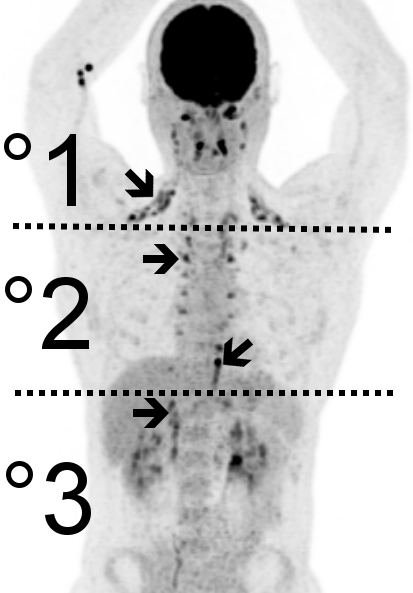
\includegraphics{Figure_grading.png} Figure 1: Maximum intensity
projection PET image depicting a grade 3 activation with lines
demarcating the different discriminative depots as proposed in {[}10{]}.
Brown fat exhibits a cranio-caudal activation pattern. In other words,
the more caudally the brown fat is activated, the higher the overall and
maximum glucose uptake.

\pagebreak

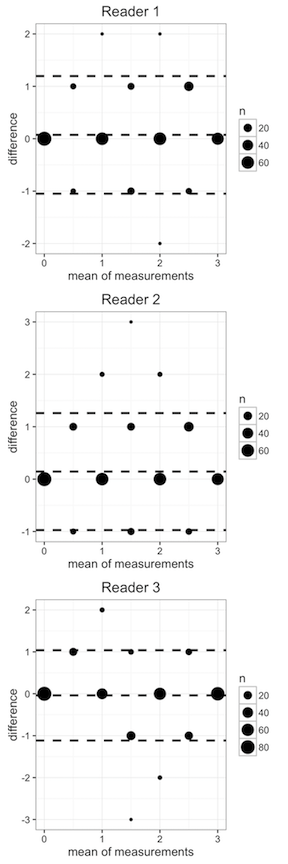
\includegraphics{Figure_BlandAltman.png} Figure 2: Bland-Altman plots of
the three readers. The size of the dots represent the number of cases.
The Figures show a slight overestimation by readers 1 and 2 (top and
middle) and underestimation by reader 3 (bottom). However, the majority
of misclassified cases were only one grade above or below the reference
grade.

\pagebreak

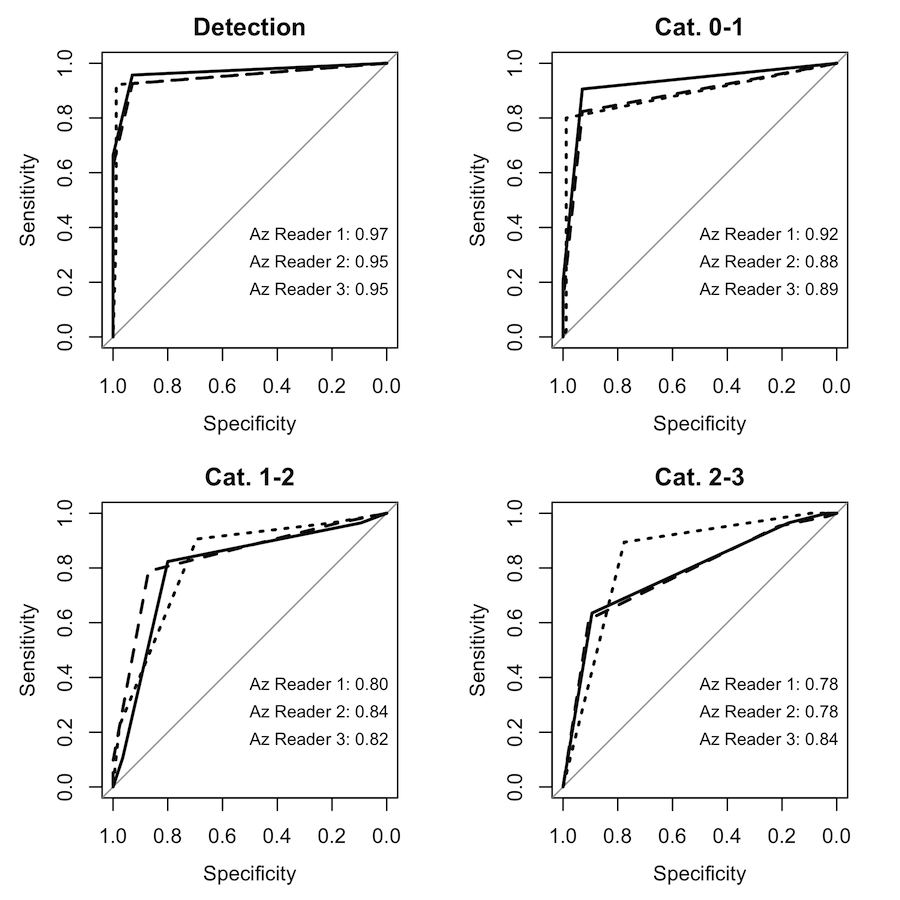
\includegraphics{Figure_ROC.png} Figure 3: ROC curves for brown fat
detection (top left) and for the distinction between the different
categories. Note the decreasing accuracy for the higher grades. The
solid line represents Reader 1, the dashed line Reader 2 and the dotted
line reader 3.

\pagebreak

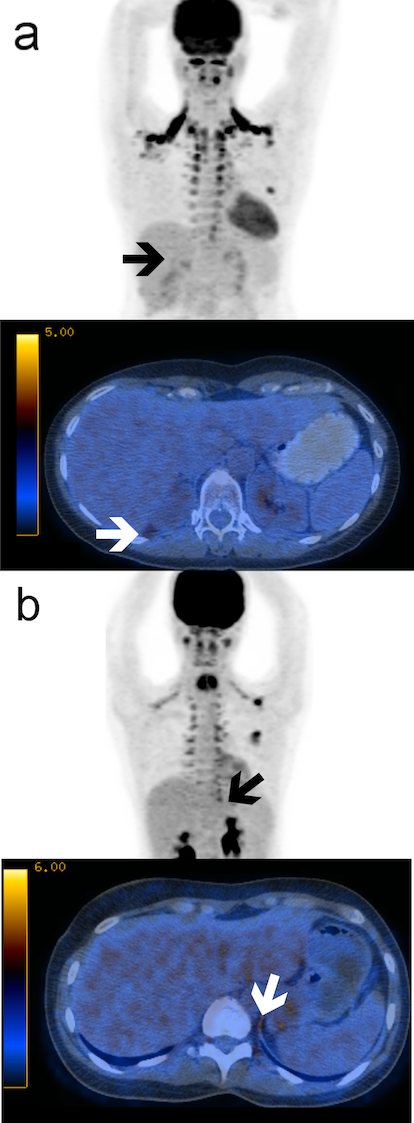
\includegraphics{Figure_examples.png} Figure 4: a) The suprarenal brown
fat in this 59 y/o female patient exhibited only very subtle FDG uptake
(arrow), which was missed by 2 readers who falsely graded the patient as
grade 2. b) In this 29 y/o female patient, muscle activity from the crus
of the diaphragm (arrow) in the vicinity of the suprarenal fat pad led 2
readers to grade the activation too high (grade 3).

\pagebreak

\subsection{Tables}\label{tables}

\begin{longtable}[]{@{}lllll@{}}
\toprule
& BAT & BAT.R1 & BAT.R2 & BAT.R3\tabularnewline
\midrule
\endhead
BAT & 1 & 0.86 (0.83-0.9) & 0.86 (0.82-0.9) & 0.89
(0.85-0.92)\tabularnewline
BAT.R1 & 0.86 (0.83-0.9) & 1 & 0.88 (0.85-0.92) & 0.87
(0.84-0.91)\tabularnewline
BAT.R2 & 0.86 (0.82-0.9) & 0.88 (0.85-0.92) & 1 & 0.83
(0.79-0.88)\tabularnewline
BAT.R3 & 0.89 (0.85-0.92) & 0.87 (0.84-0.91) & 0.83 (0.79-0.88) &
1\tabularnewline
\bottomrule
\end{longtable}

Table 1: Weighted Cohen kappa values for the three readers and the
reference reader.

\begin{longtable}[]{@{}lll@{}}
\toprule
Reference & Reader.1 & Reader.2\tabularnewline
\midrule
\endhead
1 & 0.86 (0.82-0.89) & 0.86 (0.82-0.89)\tabularnewline
0.86 (0.82-0.89) & 1 & 0.88 (0.84-0.91)\tabularnewline
0.86 (0.81-0.89) & 0.88 (0.84-0.91) & 1\tabularnewline
0.89 (0.85-0.92) & 0.87 (0.84-0.9) & 0.83 (0.78-0.87)\tabularnewline
\bottomrule
\end{longtable}

Table 2: Concordance correlation coefficients for the three readers and
the reference reader.

\begin{longtable}[]{@{}lllll@{}}
\toprule
& BAT & BAT.R1 & BAT.R2 & BAT.R3\tabularnewline
\midrule
\endhead
BAT & 1 & 0.93 (0.91-0.94) & 0.92 (0.9-0.94) & 0.94
(0.93-0.95)\tabularnewline
BAT.R1 & 0.93 (0.91-0.94) & 1 & 0.94 (0.92-0.95) & 0.93
(0.92-0.95)\tabularnewline
BAT.R2 & 0.92 (0.9-0.94) & 0.94 (0.92-0.95) & 1 & 0.91
(0.88-0.93)\tabularnewline
BAT.R3 & 0.94 (0.93-0.95) & 0.93 (0.92-0.95) & 0.91 (0.88-0.93) &
1\tabularnewline
\bottomrule
\end{longtable}

Table 3: Intraclass correlation coefficients for the three readers and
the reference reader.

\pagebreak

\subsection*{References}\label{references}
\addcontentsline{toc}{subsection}{References}

\hypertarget{refs}{}
\hypertarget{ref-ncd2016trends}{}
{[}1{]} N.R.F. Collaboration, others, Trends in adult body-mass index in
200 countries from 1975 to 2014: A pooled analysis of 1698
population-based measurement studies with 19 2 million participants, The
Lancet. 387 (2016) 1377--1396.

\hypertarget{ref-mokdad2003prevalence}{}
{[}2{]} A.H. Mokdad, E.S. Ford, B.A. Bowman, W.H. Dietz, F. Vinicor,
V.S. Bales, J.S. Marks, Prevalence of obesity, diabetes, and
obesity-related health risk factors, 2001, Jama. 289 (2003) 76--79.

\hypertarget{ref-kaukua2003behav}{}
{[}3{]} J. Kaukua, T. Pekkarinen, T. Sane, P. Mustajoki, Health-related
quality of life in obese outpatients losing weight with very-low-energy
diet and behaviour modification---a 2-y follow-up study, International
Journal of Obesity. 27 (2003) 1233--1241.

\hypertarget{ref-powell2011drug}{}
{[}4{]} A. Powell, C. Apovian, L. Aronne, New drug targets for the
treatment of obesity, Clinical Pharmacology \& Therapeutics. 90 (2011)
40--51.

\hypertarget{ref-hany2002}{}
{[}5{]} T.F. Hany, E. Gharehpapagh, E.M. Kamel, A. Buck, J. Himms-Hagen,
G.K. von Schulthess, Brown adipose tissue: A factor to consider in
symmetrical tracer uptake in the neck and upper chest region, 29 (2002)
1393--1398. \url{http://link.springer.com/10.1007/s00259-002-0902-6}.

\hypertarget{ref-cypess2009bat}{}
{[}6{]} A.M. Cypess, S. Lehman, G. Williams, I. Tal, D. Rodman, A.B.
Goldfine, F.C. Kuo, E.L. Palmer, Y.-H. Tseng, A. Doria, others,
Identification and importance of brown adipose tissue in adult humans,
New England Journal of Medicine. 360 (2009) 1509--1517.

\hypertarget{ref-virtanen2009functional}{}
{[}7{]} K.A. Virtanen, M.E. Lidell, J. Orava, M. Heglind, R. Westergren,
T. Niemi, M. Taittonen, J. Laine, N.-J. Savisto, S. Enerbäck, others,
Functional brown adipose tissue in healthy adults, New England Journal
of Medicine. 360 (2009) 1518--1525.

\hypertarget{ref-bahler2016batsuv}{}
{[}8{]} L. Bahler, F. Holleman, J. Booij, J.B. Hoekstra, H.J. Verberne,
Interobserver and intraobserver variability for the assessment of brown
adipose tissue activity on 18F-fdg pet-ct, Nuclear Medicine
Communications. 37 (2016) 363--371.

\hypertarget{ref-gifford2014auto}{}
{[}9{]} A. Gifford, T.F. Towse, R.C. Walker, M.J. Avison, E.B. Welch,
Human brown adipose tissue depots automatically segmented by positron
emission tomography/computed tomography and registered magnetic
resonance images., Journal of Visualized Experiments: JoVE. (2014).

\hypertarget{ref-becker2016bat}{}
{[}10{]} A.S. Becker, H.W. Nagel, C. Wolfrum, I.A. Burger, Anatomical
grading for metabolic activity of brown adipose tissue, PloS One. 11
(2016) e0149458.

\hypertarget{ref-wickham2009ggplot2}{}
{[}11{]} H. Wickham, Ggplot2: Elegant graphics for data analysis,
Springer Science \& Business Media, 2009.

\hypertarget{ref-cohen1968weighted}{}
{[}12{]} J. Cohen, Weighted kappa: Nominal scale agreement provision for
scaled disagreement or partial credit., Psychological Bulletin. 70
(1968) 213.

\hypertarget{ref-lawrence1989concordance}{}
{[}13{]} I. Lawrence, K. Lin, A concordance correlation coefficient to
evaluate reproducibility, Biometrics. (1989) 255--268.

\hypertarget{ref-shrout1979intraclass}{}
{[}14{]} P.E. Shrout, J.L. Fleiss, Intraclass correlations: Uses in
assessing rater reliability., Psychological Bulletin. 86 (1979) 420.

\hypertarget{ref-delong1988roc}{}
{[}15{]} E.R. DeLong, D.M. DeLong, D.L. Clarke-Pearson, Comparing the
areas under two or more correlated receiver operating characteristic
curves: A nonparametric approach, Biometrics. (1988) 837--845.

\hypertarget{ref-cicchetti1977comparison}{}
{[}16{]} D.V. Cicchetti, J.L. Fleiss, Comparison of the null
distributions of weighted kappa and the c ordinal statistic, Applied
Psychological Measurement. 1 (1977) 195--201.

\hypertarget{ref-kaushik2015estimation}{}
{[}17{]} A. Kaushik, A. Jaimini, M. Tripathi, M. D'Souza, R. Sharma, A.
Mondal, A.K. Mishra, B.S. Dwarakanath, Estimation of radiation dose to
patients from 18FDG whole body pet/ct investigations using dynamic pet
scan protocol, The Indian Journal of Medical Research. 142 (2015) 721.

\hypertarget{ref-webb2015glucose}{}
{[}18{]} R.L. Webb, E. Landau, D. Klein, J. DiPoce, D. Volkin, J.
Belman, N. Voutsinas, A. Brenner, Effects of varying serum glucose
levels on 18F-fdg biodistribution, Nuclear Medicine Communications. 36
(2015) 717--721.

\hypertarget{ref-burger2012repeatability}{}
{[}19{]} I.A. Burger, D.M. Huser, C. Burger, G.K. von Schulthess, A.
Buck, Repeatability of fdg quantification in tumor imaging: Averaged
suvs are superior to suv max, Nuclear Medicine and Biology. 39 (2012)
666--670.

\hypertarget{ref-burger2014pet}{}
{[}20{]} I.A. Burger, H.A. Vargas, A. Apte, B.J. Beattie, J.L. Humm, M.
Gonen, S.M. Larson, C.R. Schmidtlein, PET quantification with a
histogram derived total activity metric: Superior quantitative
consistency compared to total lesion glycolysis with absolute or
relative suv thresholds in phantoms and lung cancer patients, Nuclear
Medicine and Biology. 41 (2014) 410--418.

\hypertarget{ref-lopez1988amino}{}
{[}21{]} F. López-Soriano, J. Fernández-López, T. Mampel, F. Villarroya,
R. Iglesias, M. Alemany, Amino acid and glucose uptake by rat brown
adipose tissue. effect of cold-exposure and acclimation, Biochemical
Journal. 252 (1988) 843--849.

\hypertarget{ref-cypess2015activation}{}
{[}22{]} A.M. Cypess, L.S. Weiner, C. Roberts-Toler, E.F. Elía, S.H.
Kessler, P.A. Kahn, J. English, K. Chatman, S.A. Trauger, A. Doria,
others, Activation of human brown adipose tissue by a
\(\beta\)3-adrenergic receptor agonist, Cell Metabolism. 21 (2015)
33--38.

\end{document}


